% --------------------------------------
% Document Class
% --------------------------------------
\documentclass{article}
% --------------------------------------



% --------------------------------------
% Use Package
% --------------------------------------

% french, english
\usepackage[francais]{babel}

% font, french accent
\usepackage[utf8]{inputenc} 
\usepackage[T1]{fontenc} 

% page layout
\usepackage{geometry}

% hypertext link
\usepackage[pdfpagelabels]{hyperref}

\usepackage{graphicx}
\usepackage{float}
\usepackage{verbatim}
\usepackage{fancyhdr}
\usepackage{amsmath}
\usepackage{listings}


% include pdf
\usepackage[final]{pdfpages}


% --------------------------------------



% --------------------------------------
% Page setting
% --------------------------------------
%\pagestyle{empty}
\setlength{\headheight}{15pt}

\setcounter{secnumdepth}{3}
\setcounter{tocdepth}{2}

\makeatletter
\@addtoreset{chapter}{part}
\makeatother 

\hypersetup{         % parametrage des hyperliens
  colorlinks=true,      % colorise les liens
  breaklinks=true,      % permet les retours à la ligne pour les liens trop longs
  urlcolor= blue,       % couleur des hyperliens
  linkcolor= black,     % couleur des liens internes aux documents (index, figures, tableaux, equations,...)
  citecolor= green      % couleur des liens vers les references bibliographiques
}

% --------------------------------------

% --------------------------------------
% Information
% --------------------------------------
\title{Compte-rendu TP1 TI : Sources lumineuses}
\author{Elliot VANEGUE et Gaëtan DEFLANDRE}
% --------------------------------------

\definecolor{myColor}{rgb}{0.5, 0.1, 0.75}

% --------------------------------------
% Begin content
% --------------------------------------
\begin{document}
  % for listing
  \lstset{
    language=Scilab,
    commentstyle=\color{myColor}
    }

  % Set language to english
  \selectlanguage{francais}

  % Start the page counting
  \pagenumbering{arabic}

  \maketitle
  
  \mbox{}
  \newpage
  \clearpage
  
  \section{Introduction}
  Nous allons, dans ce premier TP, étudier l'éclairement de différent type
  de source lumineuse via l'outils Scilab. Le but est de trouver l'emplacement
  de plusieurs source lumineuse afin que l'éclairement d'une surface soit homogène.
  
  \section{Eclairement d'une source ponctuelle isotrope}
  Une source ponctuelle isotrope est une surface lumineuse dont l'intensité lumineuse
  est la même dans toutes les directions. Avec cette définition nous allons pouvoir
  calculer les valeurs d'éclairement pour une surface.\\
  
  Nous avons modifié le code en exemple afin de calculer les valeurs d'éclairement de 
  chaque élément de la surface par une source lumineuse isotrope. Nous obtenons le code 
  suivant :
  
  \begin{lstlisting}
  // Définition des échantillons sur un axe
  axe = [0:99] / 100 + 5e-3;
  // Définition des éléments de surface
  x = ones (1:100)' * axe;
  y = axe' * ones (1:100);
  // Position de la source -> sur le plan
  xs = 0.5;
  ys = 0.5;

  // Calcul de la distance
  d = sqrt ((x - xs).^2 + (y - ys).^2);

  // Puissance
  Phi=100;

  // Intensite energetique
  I0=Phi/2/%pi;

  // Hauteur
  h= 0.5;

  // Eclairement
  e = I0 * (h .* ((h^2 + d.^2).^(-3/2)));
  plot3d (axe, axe, e);
  imshow (e/max(e));

  \end{lstlisting}
  
  Avec ce calcul nous obtenons une courbe comme celle-ci :
  
  \begin{center}
    \begin{figure}[!h]
      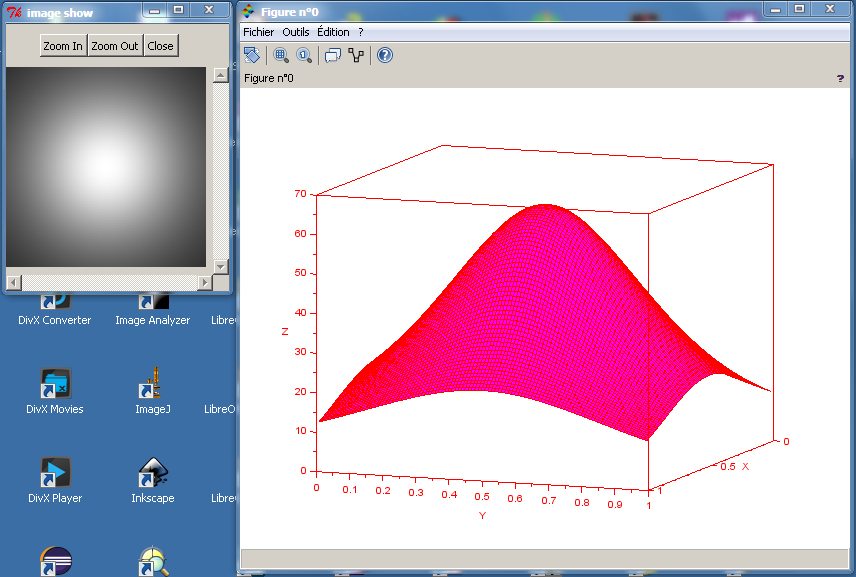
\includegraphics[width=15cm]{../isotrope.PNG}
      \caption{Graphique de la répartition de la lumière d'une source isotrope}
    \end{figure}
  \end{center}
  
  Sur ce graphique, nous pouvons voir que la lumière est plus intense sur la surface juste
  en dessous de la source lumineuse. Puis, l'éclairement reçu par la surface diminu sur les 
  bords de la surface.

  \section{Eclairement d'une source ponctuelle lambertienne}
  Une source lambertienne adopte un schéma un peu différent d'une source ponctuelle isotrope.
  Cette source aura schéma comme celui-ci :
  
  \begin{figure}[!h]
    \begin{center}
      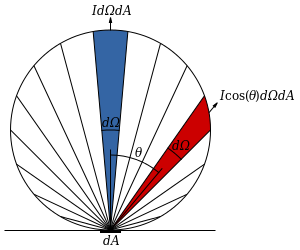
\includegraphics[width=10cm]{../Lambert_Cosine_Law_1.png}
      \caption{Représentation d'une source lumineuse isotrope lambertienne}
    \end{center}
  \end{figure}
  
  \newpage
  
  Nous avons à nouveau modifié le code afin de prendre en compte cette dispersion de la 
  lumière. Nous obtenons le calcul suivant :
  $ e = I0 * ((h^2) .* ((h^2 + d.^2).^(2)).^(-1)) $
  
  % TODO a revoir
  Ici nous voyons que l'exposant du dénominateur à changé car pour une source lambertienne 
  l'angle theta est pris deux fois. Une fois pour le départ du rayon lumineux et une second 
  fois pour ...\\
  
  Ce calcul nous donne une courbe avec une pente plus importante car la lumière éclaire moins
  les bords de la surface par rapport à une source ponctuelle isotrope.\\
  
  \begin{figure}[!h]
    \begin{center}
      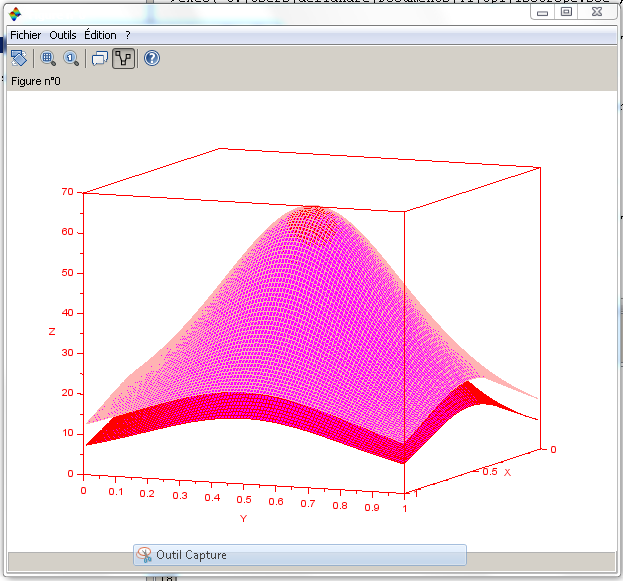
\includegraphics[width=10cm]{../iso_lamb.PNG}
      \caption{Graphique des sources ponctuelle (rose claire) et lambertienne (rose foncé)}
    \end{center}
  \end{figure}
  
  \newpage
  
  \section{Eclairement d'une grille de source ponctuelle}
    
\end{document}